\documentclass{homeworg}
\usepackage{threeparttable}
\usepackage{lscape}
\usepackage{natbib}
\usepackage{graphicx}
\usepackage{listings}
\usepackage{subfigure}
\usepackage{booktabs}

\title{Bayesian Statistics HW-2}
\author{Weijia Zhao}



\begin{document}
\maketitle

\exercise 
\textbf{k-out-of-n and Weibull Lifetime} \\
$\mathbb{P}(T\geq t)=e^{-\lambda t^r},t\geq 0, n=8, r=\frac{3}{2}, \lambda=\frac{1}{10}$ \\
(a) At time $t=3$, for any one of the component, the probability that it works is given by 
\begin{align*}
P_3=\mathbb{P}(T\geq 3)=e^{-\frac{1}{10}*3^{\frac{3}{2}}}
\end{align*}
The probability that the 4-out-of-8 system is still operational is given by 
\begin{align*}
Q_1&=\tbinom{8}{8}P_3^8(1-P_3)^0+\tbinom{8}{7}P_3^7(1-P_3)^1+\tbinom{8}{6}P_3^6(1-P_3)^2+\tbinom{8}{5}P_3^5(1-P_3)^3+\tbinom{8}{4}P_3^4(1-P_3)^4\\
&=0.818094
\end{align*}
(a) At time $t=3$, the unconditional probability that there are exactly 5 components operational is given by 
\begin{align*}
Q=\tbinom{8}{5}P_3^5(1-P_3)^3=0.277351
\end{align*}
Thus conditional on that the system was found operational at time t=3, the probability that exactly 5 components were operational is given by 
\begin{align*}
Q_2=\frac{Q}{Q_1}=0.339021
\end{align*}

\exercise 
\textbf{Precision of Lab Measurements} \\
$$ f(x)=\left\{
\begin{aligned}
\frac{3x^2}{16} &, & -2\leq x \leq 2\\
0 &,& \text{else}
\end{aligned}
\right.
$$
(a) The probability that a randomly chosen measurement can be classified as accurate is given by 
\begin{align*}
Q_1=\int_{-0.5}^{0.5} \frac{3x^2}{16}dx=0.015625=\frac{1}{64}
\end{align*}
(b) For $x\in [-2,2]$, the cumulative distribution is given by 
\begin{align*}
F(x)=\int_{-2}^{x}f(u)du=\int_{-2}^{x}\frac{3u^2}{16}du=\frac{3}{16}(\frac{8}{3}+\frac{x^3}{3})
\end{align*}
Thus the cumulative distribution function is given by 
$$ F(x)=\left\{
\begin{aligned}
0 &, &  x \leq -2\\
\frac{3}{16}(\frac{8}{3}+\frac{x^3}{3}) &,& -2<x<2 \\
1 &,& x\geq 2
\end{aligned}
\right.
$$
Below is the plot of cumulative distribution function between [-5,5] 
\begin{figure}[h]
\centering
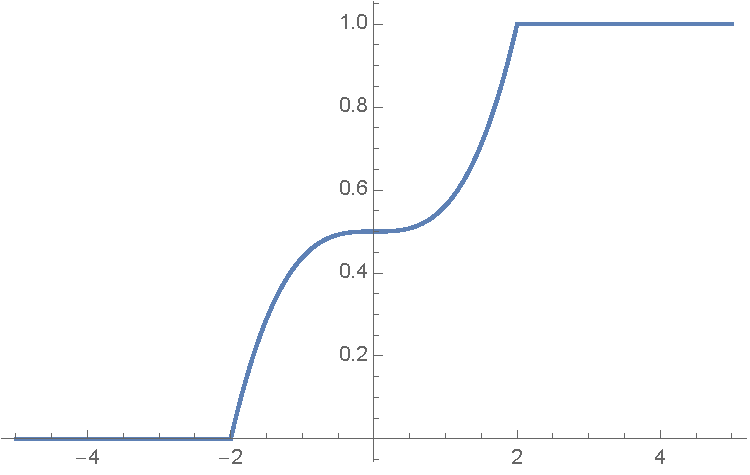
\includegraphics[]{q2_1.pdf}
\end{figure}
(c)  The mean of Y is given by 
\begin{align*}
\mathbb{E}[Y]&=\int_{-2}^{2}x^2f(x)dx=\int_{-2}^{2}\frac{3x^4}{16}dx=\frac{12}{5}=2.4
\end{align*}
Thus the mean of Y is $\frac{12}{5}$, representing an expected loss of $\frac{12}{5}$ thousand dollars. \footnote{In case we still follow the definition from (a) (this is something brought up at edstem and I do not really like this definition...) and ignore the loss caused by measurement error when the measurement is considered to be accurate (i.e. $|X|<0.5$), the mean will be given by 
	\begin{align*}
	\mathbb{E}[Y]&=\int_{-2}^{-0.5}\frac{3x^4}{16}dx+\int_{0.5}^{2}\frac{3x^4}{16}dx=2.39766
	\end{align*}\\}

(d) The probability that the loss is less than $\$3$ is equivalent to the probability that $X^2\leq \frac{3}{1000}$
\begin{align*}
\mathbb{P}=\int_{-\sqrt{\frac{3}{1000}}}^{\sqrt{\frac{3}{1000}}}\frac{3x^2}{16}dx=\frac{3\sqrt{\frac{3}{10}}}{80000}=2.05396*10^{-5}
\end{align*}
Or if we mean less than $\$3000$ actually, the probability is equivalent to the probability that $X^2\leq 3$, which is 
\begin{align*}
\mathbb{P}=\int_{-\sqrt{3}}^{\sqrt{3}}\frac{3x^2}{16}dx=\frac{3\sqrt{3}}{8}=0.649519
\end{align*}



\exercise 
\textbf{2-D Density Tasks} \\
$$ f(x,y)=\left\{
\begin{aligned}
x+y &, & 0\leq x\leq 1; 0\leq y\leq 1\\
0 &,& \text{else}
\end{aligned}
\right.
$$

(a) For $x\in [0,1]$, the marginal distribution is given by 
\begin{align*}
f_x(x)=\int_{0}^{1} (x+y) dy=x+\frac{1}{2}
\end{align*}
For $x\notin[0,1]$, the marginal distribution is 0. Thus
$$ f_x(x)=\left\{
\begin{aligned}
x+\frac{1}{2} &, & 0\leq x,y\leq 1\\
0 &,& \text{else}
\end{aligned}
\right.
$$

(b) When $x\in [0,1]$, the conditional density $f(y|x)=\frac{x+y}{x+\frac{1}{2}}$ 
$$ f(y|x)=\left\{
\begin{aligned}
\text{Not possible} &, & x\notin [0,1]\\
\frac{x+y}{x+\frac{1}{2}} &,& x\in [0,1], y\in [0,1]\\
0 &,&x\in [0,1], y\notin [0,1]
\end{aligned}
\right.
$$

\exercise 
\textbf{From the first page of Rand's book} \\

The likelihood of the sample is given by 
\begin{align*}
f(u_1,....,u_{34})=\Pi_{i=1}^{34}\frac{1}{\theta}\mathbb{I}_{\theta>u_i}=\theta^{-34}\mathbb{I}_{\theta>M}, M=0.54876
\end{align*}
Prior on $\theta$ is given by $\pi(\theta)=\frac{1}{\theta}\mathbb{I}_{\theta>0}$. Thus the joint distribution:
\begin{align*}
\pi(\theta|\{u_1,....,u_{34}\})&\propto \theta^{-34}\mathbb{I}_{\theta>M}*\frac{1}{\theta}\mathbb{I}_{\theta>0} \\
&=\theta^{-35}\mathbb{I}_{\theta>M}
\end{align*}
Given that posterior belongs to Pareto family with density $\frac{\alpha c^\alpha}{\theta^{\alpha+1}}\mathbb{I}_{\theta>c}$, we have $c=max\{M,0\}=0.54876$, $\alpha=34$ and the posterior density is $\frac{34 *0.54876^{34}}{\theta^{35}}\mathbb{I}_{\theta>0.54876}$\\

(b) As the expectation of the Pareto distribution is $\frac{\alpha*c}{\alpha-1}=\frac{34*0.54876}{33}=0.565389$. With CDF function to be $F(\theta)=[1-(\frac{c}{\theta})^\alpha]\mathbb{I}_{\theta>c}$, the left cutoff of the equitailed credible set is given by $[1-(\frac{c}{\theta_L})^\alpha]\mathbb{I}_{\theta_L>c}=0.025$, thus $\theta_L=0.549169$. Similarly, the right cutoff of the equitailed credible set is given by $[1-(\frac{c}{\theta_H})^\alpha]\mathbb{I}_{\theta_H>c}=0.975$, thus $\theta_H=0.611648$. Thus the 95\% credit set is given by [0.549169,0.611648] The true value of parameter is in the credible set.
%\setlength\bibsep{0pt}
%\bibliographystyle{apalike}
%\bibliography{hw1}


%\lstinputlisting[language=Python]{replication.py}
%\lstinputlisting[]{Untitled.do}
\newpage
\textbf{Appendix}
Mathematica code for Q2:\\

Plot[Piecewise[\{\{0, x < -2\}, \{3/16 (8/3 + x\^3/3), x >= -2 \&\& x <= 2\}, \{1, x > 2\}\}], \{x, -5, 5\}]
\end{document}








